\documentclass{pre-tfg}

\usepackage{listings}
\usepackage{formular}
\usepackage[pdftex]{graphicx}
\usepackage{afterpage}
\usepackage{longtable}
\usepackage[]{pdfpages}

\showhelp  % comenta o borra para eliminar ayudas

\title{Implantación de un sistema de integración continua en una metodología consolidada}
\author{Julio Alberto Fernández Guerrero}
\advisorFirst{Dr. Miguel Ángel Laguna Lobato}
\advisorDepartment{DEPARTAMENTO DE TECNOLOGÍAS Y SISTEMAS DE INFORMACIÓN}
\advisorSecond{Dr. Manuel Ángel Serrano Martín}
\intensification{INGENIERÍA DEL SOFTWARE}
\docdate{2017}{Marzo}


\DeclareGraphicsExtensions{.pdf,.png,.jpg}

\usepackage{color}
\definecolor{gray97}{gray}{.97}
\definecolor{gray75}{gray}{.75}
\definecolor{gray45}{gray}{.45}

\lstset{ frame=Ltb,
     framerule=0pt,
     aboveskip=0.5cm,
     framextopmargin=3pt,
     framexbottommargin=3pt,
     framexleftmargin=0.4cm,
     framesep=0pt,
     rulesep=.4pt,
     backgroundcolor=\color{gray97},
     rulesepcolor=\color{black},
     %
     stringstyle=\ttfamily,
     showstringspaces = false,
     basicstyle=\small\ttfamily,
     commentstyle=\color{gray45},
     keywordstyle=\bfseries,
     %
     numbers=left,
     numbersep=15pt,
     numberstyle=\tiny,
     numberfirstline = false,
     breaklines=true,
   }

% minimizar fragmentado de listados
\lstnewenvironment{listing}[1][]
   {\lstset{#1}\pagebreak[0]}{\pagebreak[0]}

\lstdefinestyle{consola}
   {basicstyle=\scriptsize\bf\ttfamily,
    backgroundcolor=\color{gray75},
   }

\lstdefinestyle{C}
   {language=C,
   }


\renewcommand*\lstlistingname{Listado}



\begin{document}

\maketitle

\renewcommand{\thepage}{\roman{page}}
\tableofcontents

%% CREAMOS EL PAQUETE AFTER PAGE E INSERTAMOS UNA PÁGINA EN BLANCO %%
%\afterpage{\thispagestyle{empty}\null\newpage}
\newpage 

\renewcommand{\thepage}{\arabic{page}}
\setcounter{page}{1}


\section{INTRODUCCIÓN}

Madrija Consultoría, S.L., de aquí en adelante Madrija, es una empresa que se dedica a desarrollar software utilizando una metodología de gestión del ciclo de vida del desarrollo que está en fase de consolidación. Dicha metodología se basa en principios de frameworks metodológicos ágiles y las normas ISO, en concreto utiliza la ISO 12207\cite{ISO_12207}.

En lo referente a la gestión de pruebas y automatización de testing de proyecto, Madrija utiliza Maven\cite{Maven}, lo que permite un grado de automatización a nivel de proyecto, pero presenta el inconveniente de que la ejecución de dichas pruebas debe ser manual.

Para mejorar los procesos de Madrija, se propone la implantación de un  entorno de Integración Continua\cite{IC}. Estos entornos, derivados de la práctica de \textit{eXtreme Programming}\cite{XP}, XP de aquí en adelante, permiten reducir el tiempo que los desarrolladores invierten en la detección de \textit{bugs} y facilitan la identificación de errores de regresión.

Madrija es consciente de estos beneficios y por esa razón pretende mejorar y aumentar la automatización de la ejecución de testing de integración, aumentando el alcance de las pruebas a nivel de integración entre proyectos.

\section{TECNOLOGÍA ESPECÍFICA CURSADA POR EL ALUMNO}

\begin{table}[hp]
  \centering
  \label{tab:tec-especifica}
  \zebrarows{1}
  \begin{tabular}{p{0.6\textwidth}}
    \hline
    Tecnologías de la Información \\
    Computación \\
    \rowcolor{yellow} \textbf{Ingeniería del Software} \\
    Ingeniería de Computadores \\
    \hline
  \end{tabular}
    \caption{Tecnología específica cursada por el alumno}
\end{table}
\newpage
\begin{center}
\rowcolors{1}{gray!25}{white}
\begin{longtable}{p{.40\textwidth} p{.60\textwidth}}
\hline \hline
  \textbf{Competencia} & \textbf{Justificación} \\
    \hline \hline
    Capacidad para desarrollar, mantener y evaluar servicios y sistemas software que satisfagan todos los requisitos del usuario y se comporten de forma fiable y eficiente, sean asequibles de desarrollar y mantener y cumplan normas de calidad, aplicando las teorías, principios, métodos y prácticas de la Ingeniería del Software. & Este trabajo consiste en la implantación de un entorno de integración continua que garantice un alto grado de automatización de las pruebas, de manera fiable y confiable, debido a que se prevé que este entorno de integración continua trabaje con tareas críticas, y dado que se deben obtener los mismos resultados ejecutando los tests mediante el entorno de integración continua que si se realizaran de manera manual, se justifica que se hará uso de la capacidad de desarrollar, mantener y evaluar servicios y sistemas software que satisfagan todos los requisitos del usuario y se comporten de forma fiable y eficiente, que sean asequibles tanto en su desarrollo como en su mantenimiento, y que apliquen normas de calidad mediante teorías, principios y prácticas de la Ingeniería del Software.\\
    \hline\hline
    Capacidad para valorar las necesidades del cliente y especificar los requisitos software para satisfacer estas necesidades, reconciliando objetivos en conflicto mediante la búsqueda de compromisos aceptables dentro de las limitaciones derivadas del coste, del tiempo, de la existencia de sistemas ya desarrollados y de las propias organizaciones. & Se requiere analizar y comprender la metodología propia de desarrollo utilizada en Madrija, dado que se debe incorporar en la misma un entorno de integración continua. Esta modificación a la metodología, podrá suponer cambios que generen conflictos y que deban ser resueltos considerando un equilibrio entre los objetivos buscados con la integración continua y la metodología existente. Se justifica así la capacidad indicada.\\
    \hline \hline
    Capacidad de identificar y analizar problemas y diseñar, desarrollar, implementar, verificar y documentar soluciones software sobre la base de un conocimiento adecuado de las teorías, modelos y técnicas actuales. & Dadas las necesidades software que se deben satisfacer,  y la aparición de conflictos durante la implantación del entorno de integración continua, se deben implementar, verificar y documentar las solucionas software que han sido desarrolladas, para resolver los conflictos surgidos, durante el desarrollo del proyecto para su correcta implantación, justificando así que mediante la implantación del entorno de integración continua, se adquiere la capacidad de identificar y analizar problemas y diseñar, así como de desarrollar, implementar, verificar y documentar soluciones software sobre la base de un conocimiento adecuado de las teorías, modelos y técnicas habituales.\\
    \hline \hline
    Capacidad de dar solución a problemas de integración en función de las estrategias, estándares y tecnologías disponibles. & Mediante la implantanción e integración del entorno de integración continua en la metodología de desarrollo de Madrija junto con todas sus herramientas, Vagrant o VirtualBox\cite{VirtualBox} entre otras muchas, siendo necesaria la capacidad para dar solución a problemas de integración en función del conocimiento de estrategias, estándares y tecnologías disponibles.\\
    \hline \hline
\caption{Justificación de las competencias específicas abordadas en el TFG}
\end{longtable}
\end{center}

\section{OBJETIVOS}

\subsection{Objetivo principal}

\fbox{\parbox[b]{\linewidth}{\hspace{1em} El objetivo de este trabajo es analizar, diseñar e implementar un entorno de integración continua, que se adapte a la metodología, formas y prácticas de desarrollo que tiene Madrija.}}

Los subobjetivos a tratar en este trabajo son:

\begin{itemize}
\item Analizar y determinar herramientas de integración continua.
\item Adaptarse a la metodología de desarrollo.
\item Alcanzar el máximo grado de automatización posible de los tests.
\item Proponer mejoras.
\end{itemize}

\subsubsection{Analizar y determinar herramientas de integración continua}
Madrija es consciente de los beneficios de implantar un entorno de integración continua, por ello, requiere que se realice un estudio para analizar las herramientas y elegir la que más beneficie y mejor se adapte a la metodología de desarrollo de la empresa.

\subsubsection{Adaptarse a la metodología de desarrollo}

Madrija cuenta con una metodología propia de desarrollo, que será mejorada y complementada por la implantación del sistema integración continua, para ello, se debe analizar y comprender la metodología utilizada por Madrija.

\subsubsection{Alcanzar el máximo grado de automatización posible de los tests}

Madrija realiza de manera manual, utilizando Maven, las pruebas a sus proyectos lo que supone pérdidas de tiempo, además, también influye el factor humano dado que existe la posibilidad de que no se realicen dos pruebas iguales a un mismo desarrollo en un mismo test o, incluso, que haya días en los cuales no se realicen pruebas.

\subsubsection{Proponer mejoras}

Para la implantación del entorno de integración continua, Madrija, deberá realizar una serie de cambios dentro de su metodología para que dicha implantación sea factible, es decir, se debe analizar la forma en la que desarrolla Madrija y estudiar la manera más fácil mediante la cual realizar dicha implantación.

\subsection{Justificación}

Este trabajo tiene varias causas que lo justifican entre las que destacan, el ahorro de tiempo, como se ha dicho antes, Madrija realiza las pruebas a sus proyectos de manera manual, utilizando Maven, el cual automatiza una parte de las pruebas, pero necesita ser ejecutado por el equipo de desarrollo, pudiendo propiciar también fallos humanos a la hora de realizar la ejecución de dichas pruebas, ocasionando que se cometa el error de no realizar siempre las mismas pruebas al mismo desarrollo.

La necesidad de un análisis a fondo de la forma de desarrollo de la empresa para que la implantación del entorno de integración continua sea lo más factible posible.

\section{METODOLOGÍA DE DESARROLLO}
\subsection{Introducción}

En este proyecto no es posible utilizar metodologías de gestión de proyectos como proceso unificado de desarrollo o SCRUM\cite{SCRUM}, dado que este proyecto no versa sobre el desarrollo de un producto, ni tampoco sobre el desarrollo de un software y que, en cualquier caso, será realizado por una persona.

En su lugar, se procederá a modelar iterativamente utilizando una heurística, en concreto, la heurística IDEAL, y a partir de los resultados obtenidos en cada iteración se incrementa el prototipo obtenido en la última fase de cada iteración.

\subsection{Heurística IDEAL}

IDEAL fue formulada por Bransford y Stein en 1984\cite{Brans93}, incluye 5 pasos de los cuales surgen el nombre de esta metodología, \textbf{I}dentificar el problema, \textbf{D}efinir y presentar el problema, \textbf{E}xplorar las estrategias viables, \textbf{A}vanzar en las estrategias y \textbf{L}ograr la solución.

La heurística IDEAL se define como iterativa e incremental, dado que repite varias veces el proceso hasta que el problema ha sido resulto por completo, e incremental puesto que cada iteración y nuevo inicio por los pasos del ciclo va incrementando las partes del proyecto a evaluar.

Para su estudio y aplicación, realmente, en vez de en cinco fases se suelen agrupar las dos primeras en una única fase\cite{Perales94}, \textit{``Identificar y definir el problema''} tratan aspectos muy parecidos por lo que para evitar redundancias a la hora de realizar tareas se agrupan en una única fase.

\begin{figure}[!h]
\centering
   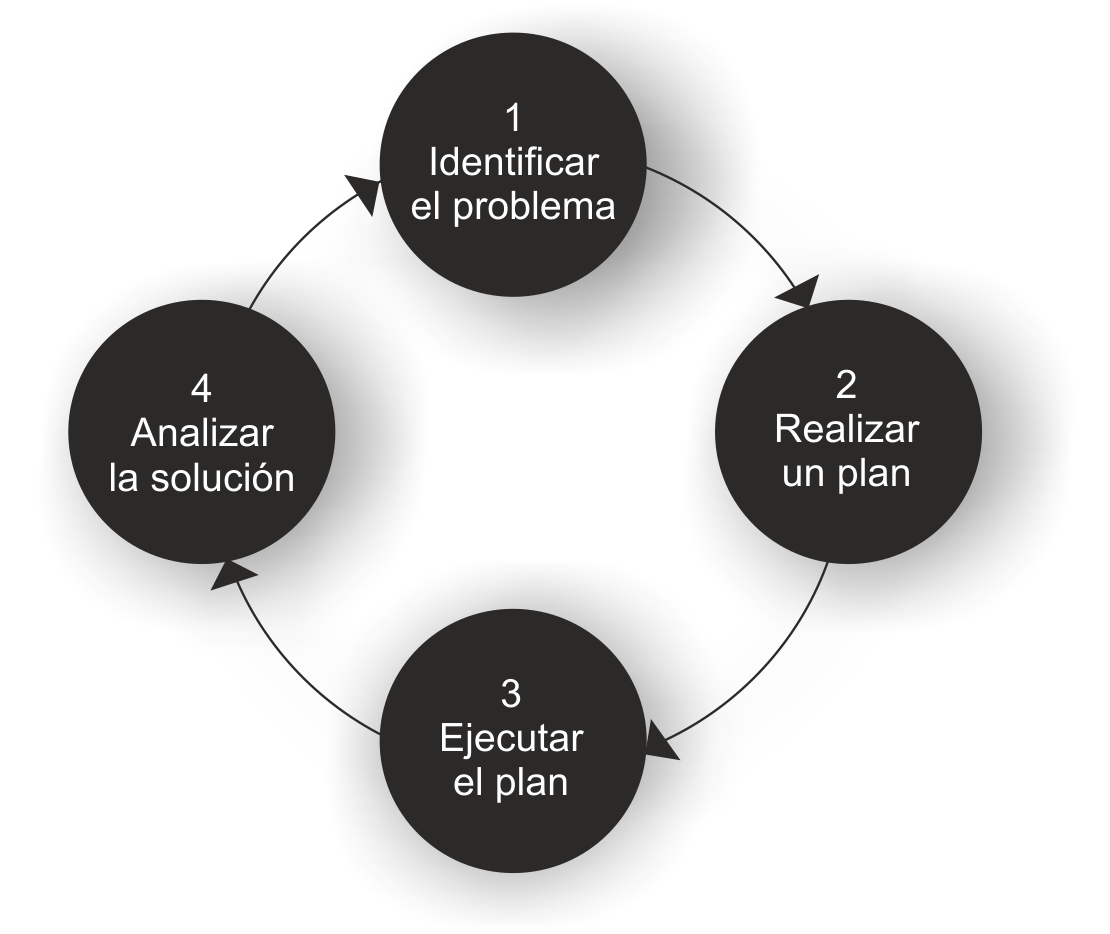
\includegraphics[width=8cm]{Ciclo_IDEAL.png}
\caption{Ciclo IDEAL}
\end{figure}

\subsubsection{Identificación del problema}

En esta primera fase del ciclo a realizar, se procede a observar y analizar el problema y se determina el resultado que se debe obtener. En concreto para este trabajo, se toma como entrada la última salida del ciclo, en este caso, el prototipo obtenido en la última fase.

\subsubsection{Realización del plan}

Se determinan los pasos y operaciones a realizar para resolver el problema planteado. Por lo general, se descompone el problema en subproblemas más pequeños para facilitar la manera de resolver dicho problema, además, introducimos la herramienta de gestión de proyectos OpenProject\cite{OpenProject}, en dicha herramienta introduciremos los pasos a seguir para resolver el problema e identificaremos las distintas versiones del proyecto, en general para este trabajo, tomaremos los test que debe superar la aplicación y se analizará la manera mediante la cual se deben superar, o se debe provocar los fallos de los tests en busca de errores.

\subsubsection{Ejecución del plan}

Se procede a la ejecución en detalle cada operación, siguiendo la especificación de pasos a seguir en OpenProject, despúes de realizarse la descomposición en subproblemas más pequeños.

\subsubsection{Analizar la solución}

Una vez resuelto el problema identificado en la primera fase, se confirma la nueva versión del prototipo del entorno de integración continua en OpenProject, además, se toman técnicas de SCRUM y se realizan reuniones al final de cada iteración con el equipo de desarrollo para ver la evloución del prototipo, se inicia de nuevo el ciclo IDEAL desde la primera fase, tomando como entrada la salida de esta última fase, es decir, la última versión del prototipo.

\section{MEDIOS A UTILIZAR}
\subsection{Medios software}

Debido a que este trabajo se realiza mediante un convenio FORTE, las herramientas a utilizar son impuestas por la empresa, en este caso, por Madrija.
\\

\begin{itemize}
\item \textbf{Sistemas operativos}
\begin{itemize}
\item \textbf{Windows 10 Home x64: }Estación de trabajo.
\item \textbf{Ubuntu Server x64: }Servidor de la empresa.
\end{itemize}
\end{itemize}

\begin{itemize}
\item \textbf{Herramientas y tecnologías para el desarrollo software}
\begin{itemize}
\item \textbf{Jenkins: }es un servidor de integración continua de código abierto. \cite{Jenkins}
\end{itemize}
\begin{itemize}
\item \textbf{Java: }lenguaje de programación y una plataforma informática comercializada por Sun Microsystems. \cite{Java}
\end{itemize}
\begin{itemize}
\item \textbf{Maven: }es una herramienta que se utiliza para construir y gestionar cualquier proyecto, y sus dependencias, basado en Java.
\end{itemize}
\end{itemize}

\begin{itemize}
\item \textbf{Control de versiones}
\begin{itemize}
\item \textbf{Git:} sistema de control de versiones de código abierto. \cite{Git}
\item \textbf{GitLab:} plataforma de desarrollo colaborativo para el alojamiento de proyectos que utilizan el sistema de control de versiones Git. \cite{GitLab}
\end{itemize}
\end{itemize}

\begin{itemize}
\item \textbf{Modelado y documentación}
\begin{itemize}
\item \textbf{\LaTeX: }es un sistema de composición de textos, orientado a la creación de documentos escritos que presenten una alta calidad tipográfica. \cite{LaTeX}
\item \textbf{Inkscape: }software para edición de imágenes basado en gráficos vectoriales. \cite{Inkscape}
\end{itemize}
\end{itemize}

\begin{itemize}
\item \textbf{Herramientas para la virtualización}
\begin{itemize}
\item \textbf{Oracle VM VirtualBox: }Oracle VM VirtualBox es un software de virtualización para arquitecturas x86/amd64.
\end{itemize}
\end{itemize}

\begin{itemize}
\item \textbf{Herramientas para la gestión del proyecto}
\begin{itemize}
\item \textbf{OpenProject:} software dedicado a la gestión de proyectos.
\end{itemize}
\end{itemize}

\subsection{Medios hardware}

\begin{itemize}
\item \textbf{PC:} Ordenador portátil HP NOTEBOOK 15-r213ns con las siguientes características hardware:
\begin{itemize}
\item Procesador Intel(R) Core(TM) i7-5500U CPU @ 2.40GHz
\item 8 GB RAM
\item HDD 1 TB
\end{itemize}
\end{itemize}

\newpage

\section{BIBLIOGRAFÍA}
\bibliographystyle{acm}
\singlespacing
\bibliography{ejemplo}
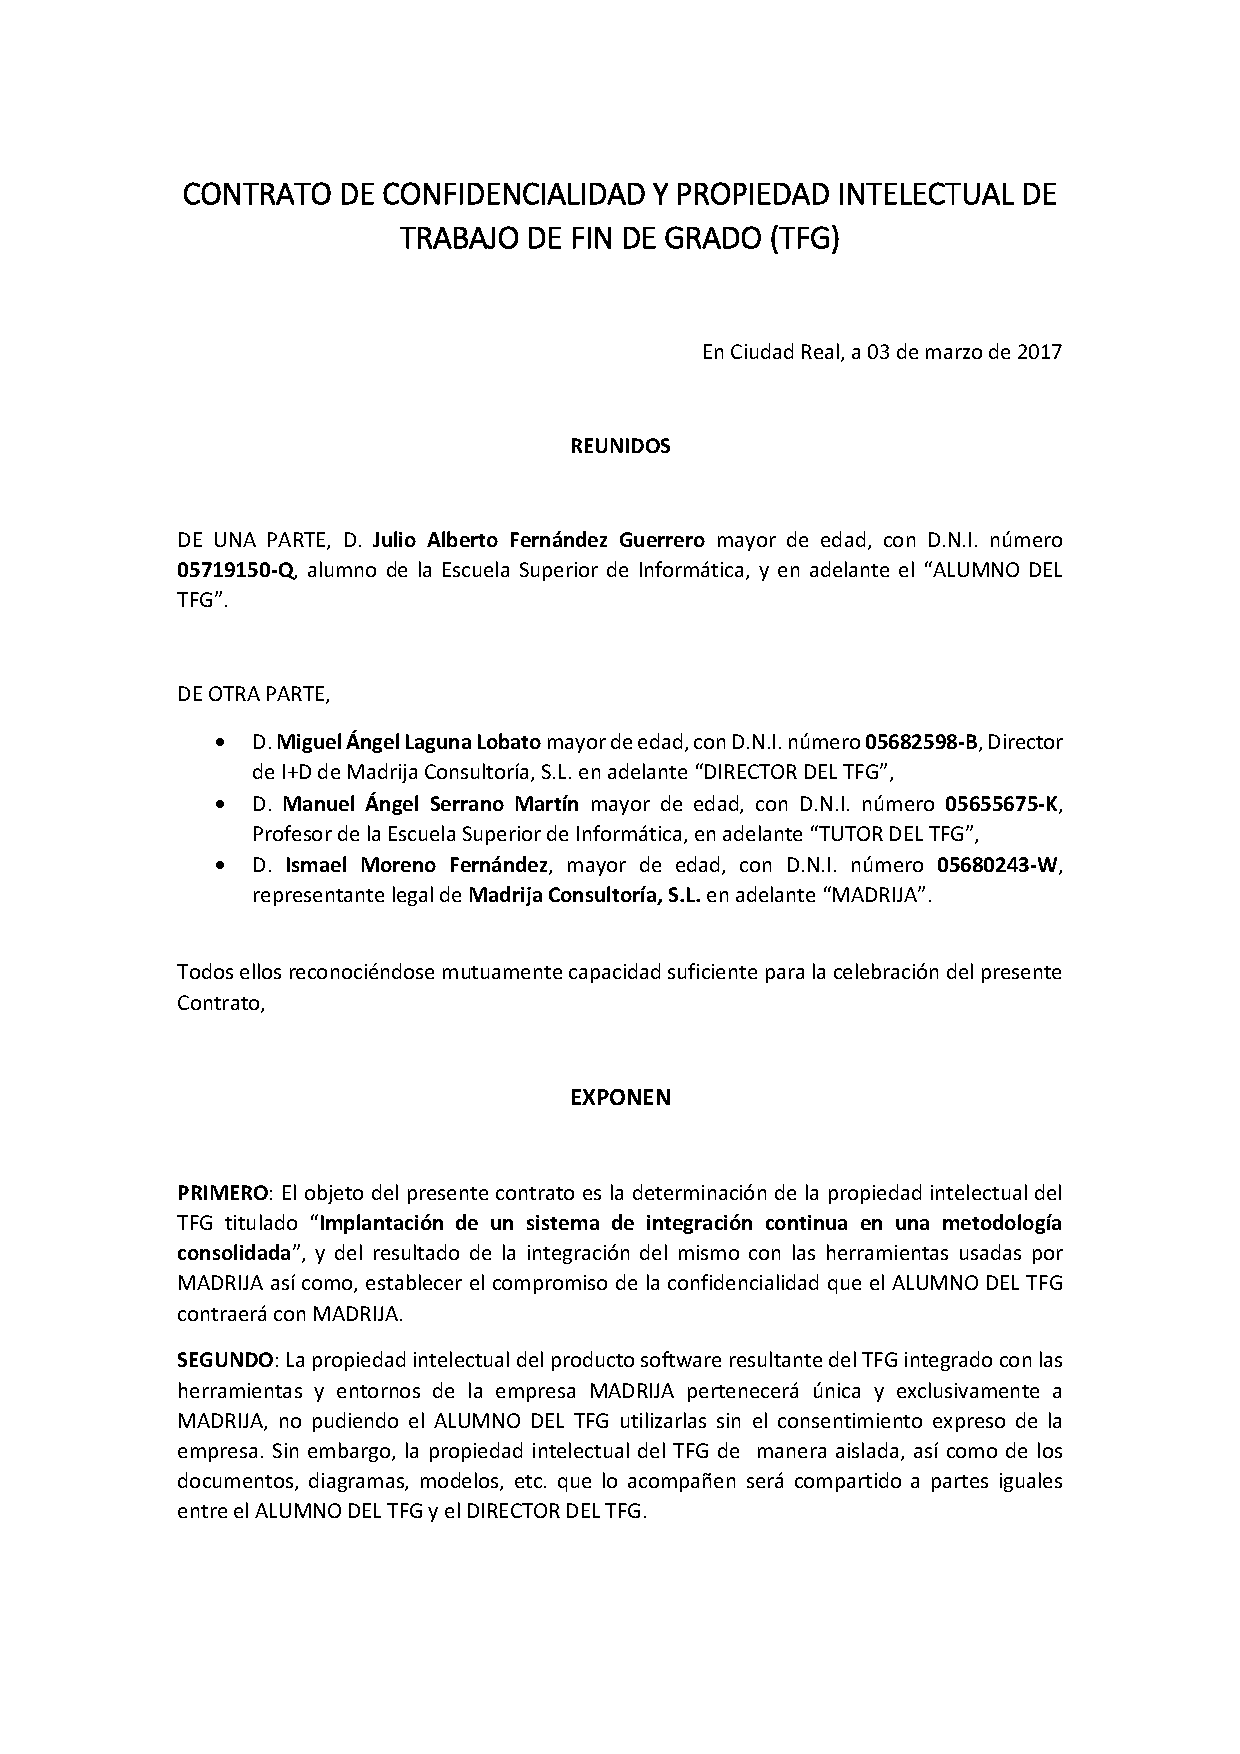
\includepdf[pages=-]{Contrato_Propiedad_Intelectual002.pdf}

\end{document}